% !TEX root = ../main.tex

\addtocontents{toc}{\protect\newpage}
\secc{Design and implementation}

\ssecc{Get familiar with survival models}

\ssecc{Preprocess data}

As it was previously stated the data needs to be preprocessed before start training with it.
This steps are required because small changes can really help in reducing the time needed to
fit the model. Also, by normalizing the data and setting variance to 1 and mean to 0 the network
can converge faster ~\cite{neural:efficient-backprop}. 
The preprocess steps are divided into three categories:
\begin{itemize}
  \item Preprocess the image data
  \item Preprocess the scalar data
  \item Generate the pairs for training
\end{itemize}

The whole preprocess task took longer than expected as many tasks required more steps than 
planned. The planned duration was 1 week and the final duration was from March 13\Th and
ended in April 11\Th so its duration was of 4 weeks. However, this wasn't as problematic as 
it could seem since the previous task was completed early.

Also, this task has been done sometimes while doing other tasks because some preprocess 
steps have been added later to improve the network's results.

\sssecc{Image data}

The imaging data in the \Gls{PMHNK} contains 671 folders, each one with the scan of one patient. 
We also have the clinical information of 661 patients, although we do not have a \gls{CT} for
each of the clinical information patients. Through the intersection of each of the two data
sources we have 544 patients with both a \gls{CT} scan and the clinical information.

However, because there was a problem in the way the \gls{CT} scan was computed we only have
the tumour annotations for 509 of the 544 patients, so the data that we can use is reduced
again. Moreover, while extracting the radiomic features only 490 of the 509 patients produce 
usable results. \textbf{490} will be the final dataset size that will be used for the next 
steps.

For all the valid patients their directory structure is the same. They contain two folders,
one with all the original scan slices and the other with the slice's tumour mask annotations. 
All the slices are in \verb|.dcm| format.
As an example, the structure for patient \texttt{FHBO0003} can be seen in \autoref{fig:hnk-raw}.

\begin{figure}
  \centering
  \begin{minipage}{0.8\textwidth}
    \begin{Verbatim}[samepage=true]
FHBO003
├── FHBO003           // Original scan
│   ├── IMG0001.dcm
│   ├── IMG0002.dcm
│   ├── ...
│   └── IMG0191.dcm
└── FHBO003-MASS      // Annotated mask
    ├── IMG0001.dcm
    ├── IMG0002.dcm
    ├── ...
    └── IMG0191.dcm
    \end{Verbatim}
  \end{minipage}
    
  \caption{Original data directory structure \label{fig:hnk-raw}}
\end{figure}

Preprocessing the image data requires multiple steps:
\begin{enumerate}
  \item Select valid directories that follow the previously stated conditions
  \item Join all the \verb|.dcm| files into a 3D \verb|numpy| array
  \item Apply gaussian filter to mask image. This is done because the mask is manually annotated
        and usually each layer does not fit perfectly with the previous one. This way a smooth
        transition between layers is ensured.
  \item Get 3D bounding box containing the tumour.
  \item Slice original image and mask with the bounding box to extract the parts only containing
        the tumour. A single bounding box is obtained.
  \item Remove extreme values, if the value of the image is smaller than -1000 or bigger than
        400 this means that this are pixels usually outside of the scanner. This happens because
        the scanner has a circular field of view but a squared image is generated instead, so 
        all the pixels outside the circle are \emph{error pixels}.
  \item Apply mask to extracted image. Since the mask only contains 1s and 0s it's as easy 
        as \verb|image *= mask|.
  \item Resize the sliced image to a size of \( 64 \times 64 \times 64 \)
  \item Normalize image by setting mean = 0 and variance = 1. It's done in the following way:
  \begin{itemize}
    \item \verb|image -= mean(image)|
    \item \verb|image /= std(image)|
  \end{itemize}
  \item Rotate the image 3 times to get 4 different versions of the scan that can be used for 
        training as data augmentation.
\end{enumerate}

\begin{figure}
  \resizebox{\textwidth}{.7\textwidth}{
    \def\customimage{5em}
\begin{tikzpicture}[node distance = 2]
    \node (P-0) at (0, 0) {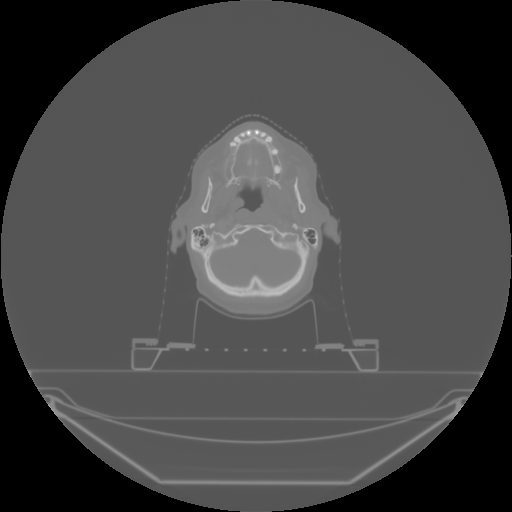
\includegraphics[width=\customimage]{images/preprocess/process_0}};
    \node [below = of P-0] (P-1) {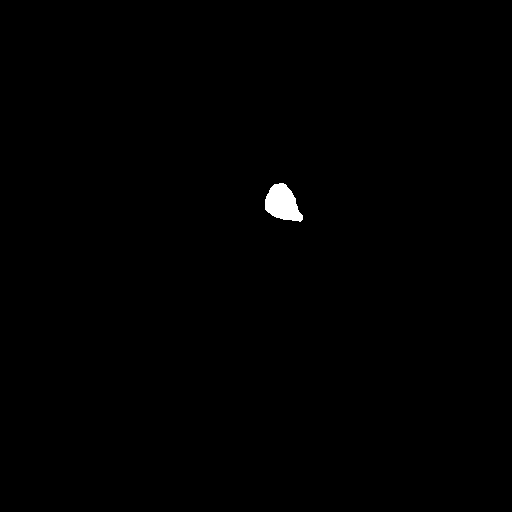
\includegraphics[width=\customimage]{images/preprocess/process_1}};

    \node [below = .2 of P-0] (text-0) {Scan};
    \node [below = .2 of P-1] (text-1) {Mask};
    
    \node [right = of P-1] (P-2-0) {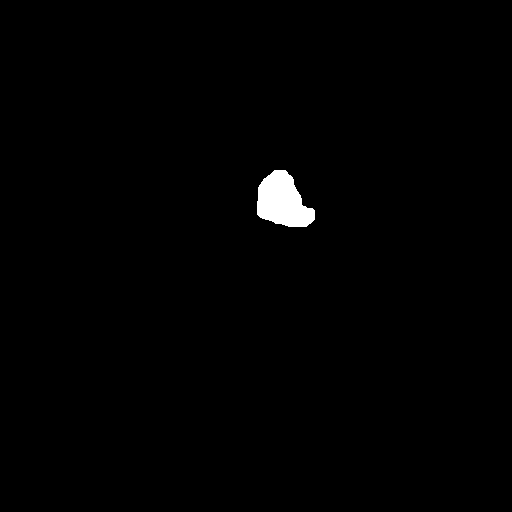
\includegraphics[width=\customimage]{images/preprocess/process_2_0}};
    \node [right = of P-2-0] (P-2-1) {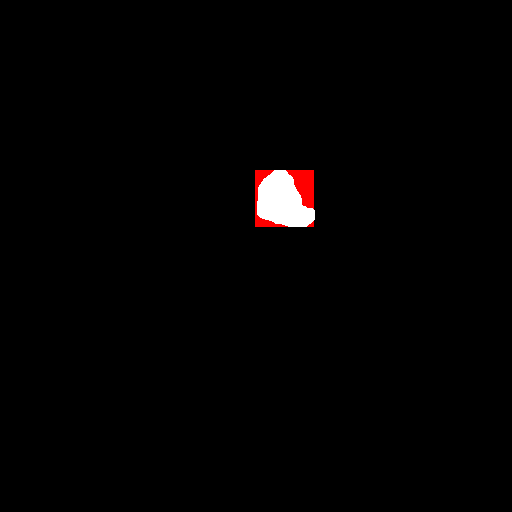
\includegraphics[width=\customimage]{images/preprocess/process_2_1}};
    \node [right = of P-2-1] (P-5) {
\includegraphics[width=\customimage]{images/preprocess/process_5}};
    
    \node [above = of P-2-1] (P-3) {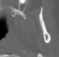
\includegraphics[width=\customimage]{images/preprocess/process_3}};
    \node [right = of P-3] (P-4) {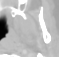
\includegraphics[width=\customimage]{images/preprocess/process_4}};

    \node [right = .5 of P-5, circle, draw] (prod) { \Large \( \times \) };
    
    \node [below = of P-5] (P-6) {
\includegraphics[width=\customimage]{images/preprocess/process_6}};
    \node [left = of P-6] (P-7) {
\includegraphics[width=\customimage]{images/preprocess/process_7}};
    \node [left = of P-7] (P-8) {
\includegraphics[width=\customimage]{images/preprocess/process_8}};

    \node [below = .2 of P-6] { \( 59 \times 57 \) px};
    \node [below = .2 of P-7] { \( 64 \times 64 \) px};
    \node [below = .2 of P-8] { \( 64 \times 64 \) px};

    \draw [-latex] (P-0) -- (P-3);
    \draw [-latex] (P-3) -- (P-4) node[midway, below, align=center] {Remove \\ extreme \\ values};
    \draw [-latex] (P-4) -| (prod);

    \draw [-latex] (P-1) -- (P-2-0) node[midway, below, align=center] {Gaussian \\ filter};
    \draw [-latex] (P-2-0) -- (P-2-1) node[midway, below, align=center] {Bounding \\ box};
    \draw [-latex] (P-2-1) -- (P-3) node[midway, right, align=center] {Slice};
    \draw [-latex] (P-2-1) -- (P-5) node[midway, below, align=center] {Slice};
    \draw [-latex] (P-5) -- (prod);

    \draw [-latex] (prod) |- (P-6) node[near end, below, align=center] {Apply \\ mask};
    \draw [-latex] (P-6) -- (P-7) node[midway, below, align=center] {
        Resize \\ \( 64 \times 64 \)
    };

    \draw [-latex] (P-7) -- (P-8) node[midway, below, align=center] {Normalize};

\end{tikzpicture}
  }

  \caption[Image pre-process pipeline]{
    Image pre-process pipeline \label{fig:preprocess}
    
    In this example the process is shown for a 2D image, all the pictures are being resized to 
    have the same size so the steps can be appreciated. The normalization step is not shown as is,
    since setting a mean of 0 and variance of 1 produces an invalid \acrshort{PNG} image, but still valid
    for \gls{ML} purposes.
  }
\end{figure}

\sssecc{Scalar data}

There are two types of scalar data:
\begin{itemize}
  \item Clinical information
  \item Radiomic features extracted from the image, regarding tumour shape, intensity, volume...
\end{itemize}

The clinical information should be anonymized as much as possible and especially if it's going
to be outside \gls{UHN}, the network of hospitals where this project is being developed.
Since this is the case, as the training will be done at \gls{CC} cluster, the unnecessary fields
are removed and only those being used are kept. Moreover, removing the unused fields
is helpful when using the data.

Originally, the clinical information provides 36 different fields. From these fields only the 
following ones are kept:
\begin{itemize}
  \item ID
  \item Age
  \item Sex
  \item Survival event. This one needs to be negated since, in the provided event, \verb|event = 1|
        means survival, but in our survival model this means death. 
  \item Survival time
\end{itemize}

The radiomic features can be extracted directly with the \emph{PyRadiomics}
\cite{medical:py-radiomics} package, but in this case they have been already extracted and stored
in a single file so we can reuse them. These features should be normalized before start training,
because otherwise the network may never converge, which indeed it happened. 

For this normalization to be valid, the mean and the standard deviation are obtained only from 
the train samples. These are different for each feature because not all the features need to 
be normalized in the same way. Afterwards, the normalization is applied to both the train 
and test samples. The mean for the test samples is never obtained, because, otherwise, the
model could have \gls{leakage}. An example of features normalization can be seen in
\autoref{fig:feature-normalization}

\begin{figure}
  \centering

  \begin{subfigure}[t]{.49\textwidth}
    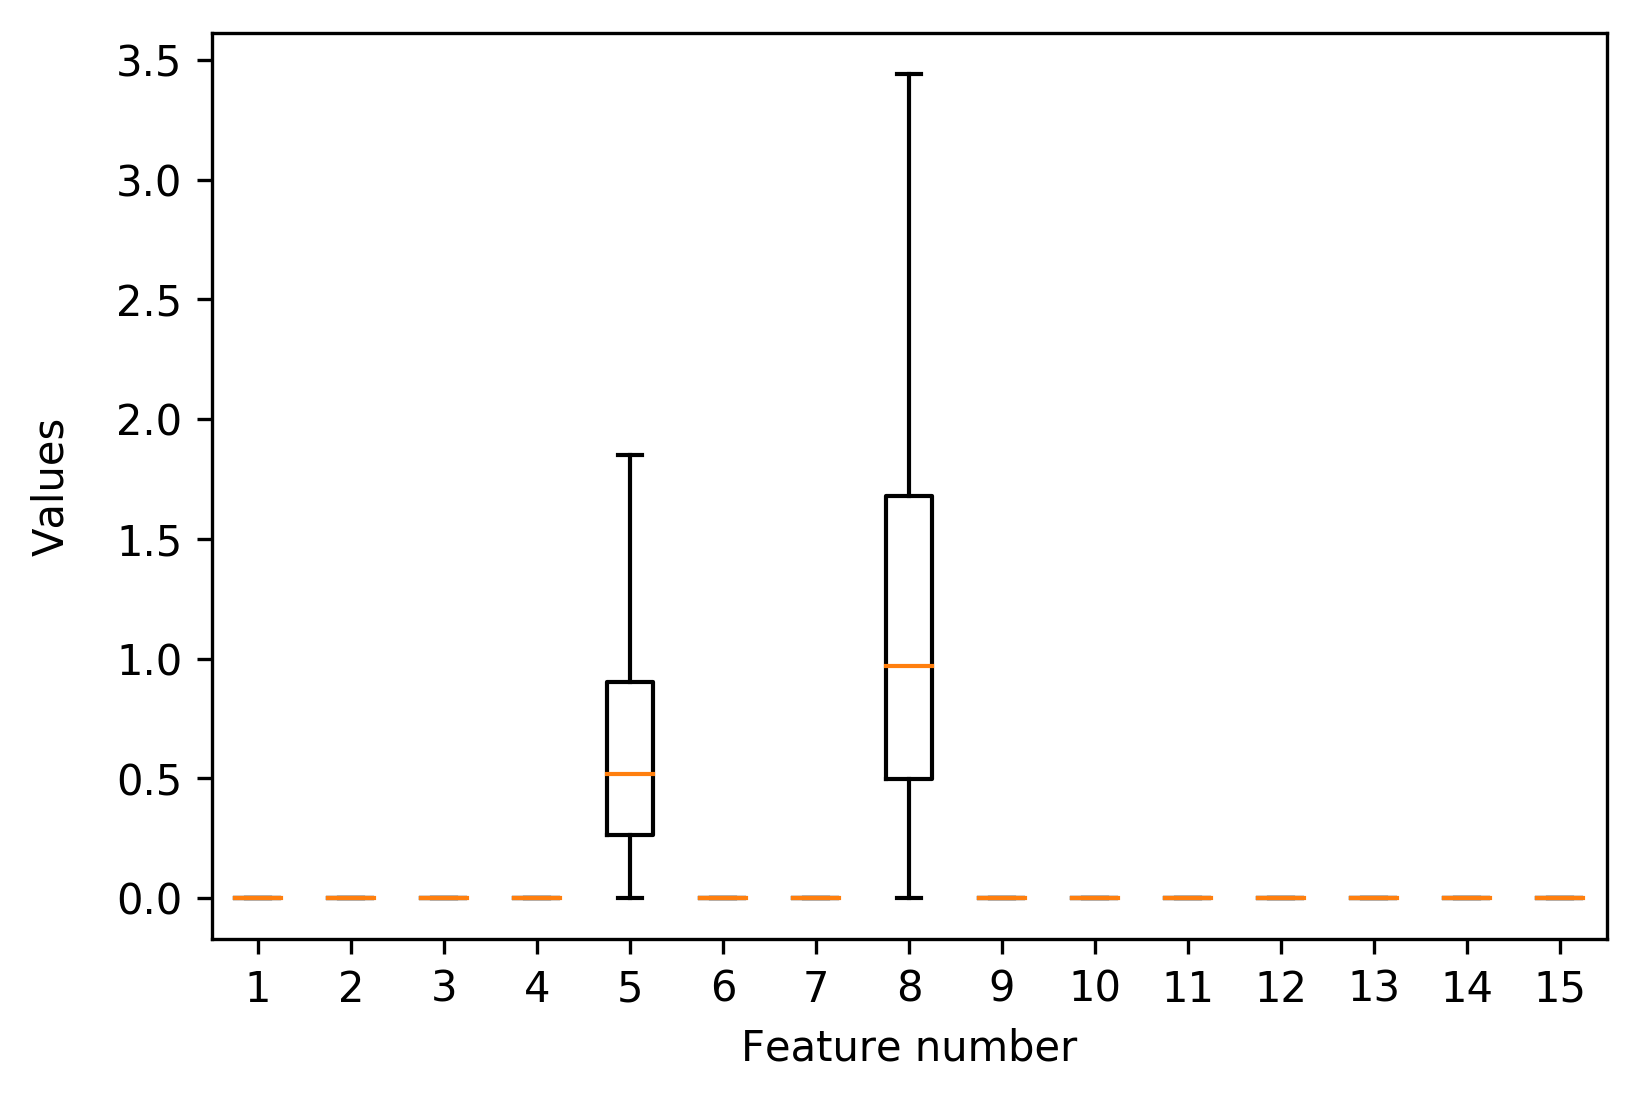
\includegraphics[width=\textwidth]{images/features_original}

    \caption{Features' box plot before normalization \label{fig:feature-normalization-before}}
  \end{subfigure}
  \hfill
  \begin{subfigure}[t]{.49\textwidth}
    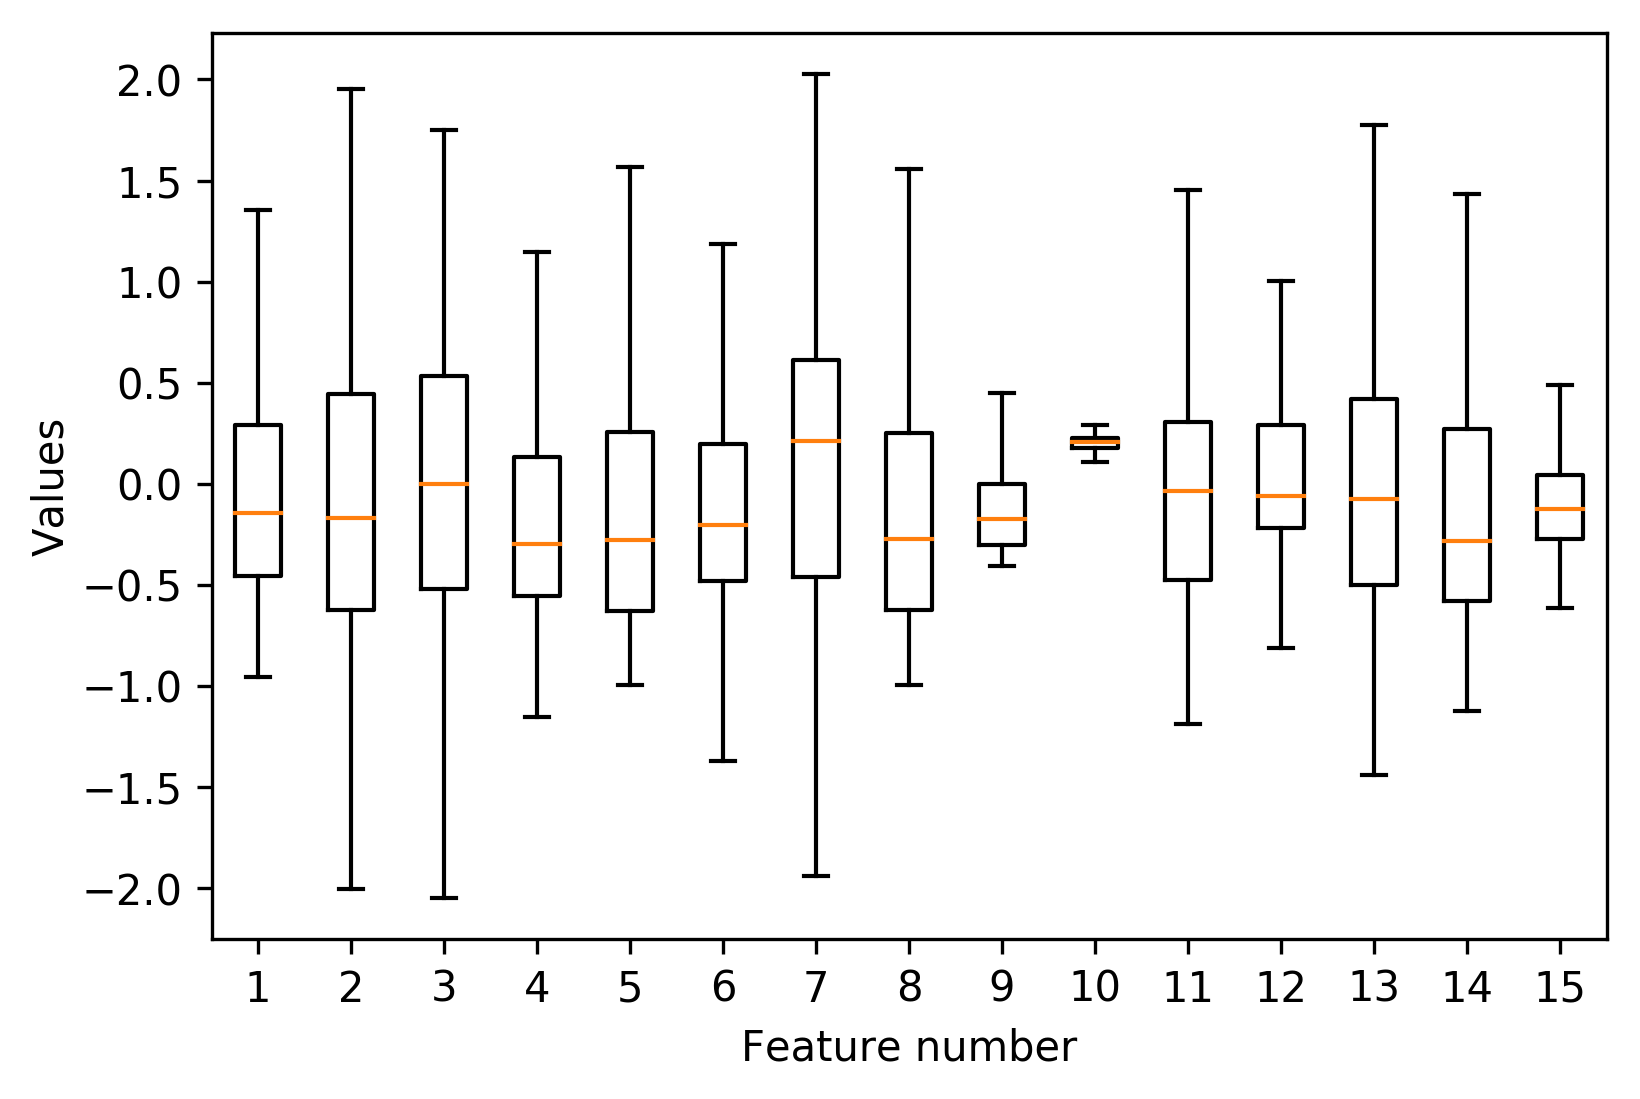
\includegraphics[width=\textwidth]{images/features_normalized}

    \caption{Features' box plot after normalization}
  \end{subfigure}

  \caption[Features normalization example]{
    Features normalization example \label{fig:feature-normalization}
    
    In this example only the first 15 of 725 features are shown for readability. 
    \autoref{fig:feature-normalization-before} shows the features before normalizing them. 
    There, many of the features are too small compared with the ones shown so only a small 
    line is drawn.
  }
  
\end{figure}


\sssecc{Pair generation}

As the siamese network is prepared to train in pairs these have to be generated before. As
it has been explained in \autoref{sec:survival} and shown in \autoref{fig:graph-ci},
for two subjects \( A \) and \( B \) a pair can only be generated if:
\begin{itemize}[noitemsep, topsep=0pt]
  \item Both of them are uncensored (\( E_A = E_B = 1\))
  \item The uncensored time of one is smaller than the censored survival time of the other
  (\( T_A < T_B | E_A = 1; E_B = 0 \))
\end{itemize}

These conditions are to be kept in mind when generating the pairs. Moreover, before starting
the train and test sets must be decided first. Once they have been generated then the pairs
can be generated too. To avoid \gls{leakage} three types of pairs will be defined and will be
used in different contexts:
\begin{description}
  \item[\Gls{train-pair}] \glsdesc*{train-pair}
  \item[\Gls{test-pair}] \glsdesc*{test-pair}
  \item[\Gls{mixed-pair}] \glsdesc*{mixed-pair}
\end{description}

When generating mixed pairs the rules are a bit different. Since the network is not supposed
to know anything about the test set elements, only uncensored elements from the train set
are used to avoid creating pairs where both elements are censored.

\begin{figure}
  \centering
  \def\customimage{5em}
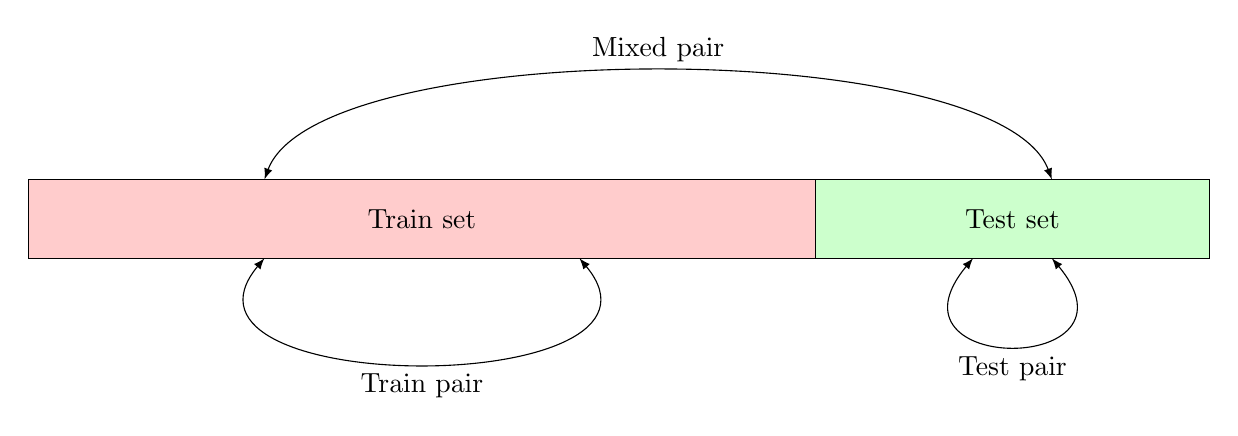
\begin{tikzpicture}
    
    \draw [fill = red!20] (0, 0) rectangle (10, 1);
    \draw [fill = green!20] (10, 0) rectangle (15, 1);

    \node at (5, .5) {Train set};
    \node at (12.5, .5) {Test set};

    \draw [bend right=130, latex-latex, looseness=1.5] (3, 0) to node [midway, below] {Train pair} (7, 0);
    \draw [bend right=130, latex-latex, looseness=5] (12, 0) to node [midway, below] {Test pair} (13, 0);
    \draw [bend left=70, latex-latex, looseness=.5] (3, 1) to node [midway, above] {Mixed pair} (13, 1);
\end{tikzpicture}
  \caption{Types of pairs generated from the test and train sets}
\end{figure}


\ssecc{Create basic siamese model}
\label{sec:basic-siamese}

The first step is to create an environment where different sisters networks can be tested
for improvements. To do so, the loss and cost functions are defined assuming a sister
network's output \( \bm{O} \) form the input \( \bm{X} \). This will be called the
\emph{basic model}.

The distance comparison used for the following siamese networks is defined comparing the 
absolute distance of the sister's output features and then applying the logistic function 
into it to get an output value \( d \in [0, 1] \). This way if it's 1 it means \( T_B > T_A \).
Future designs should implement the sister network's part for this model to work.
\begin{align*}
  \bm{O}_A &= \operatorname{sister}(\bm{X}_A) \\
  \bm{O}_B &= \operatorname{sister}(\bm{X}_B) \\
  \sigma(x) &= \frac{1}{1 + \exp(-x)} \\
  d &= \sigma(||\bm{O}_B||_2 - ||\bm{O}_A||_2) 
\end{align*}

Note that, since the output is a real number, to compute the \gls{CI} a threshold has been
set to round the real numbers to 0 or 1. The threshold value is 0,5 so if a number is 
bigger than the threshold it will be rounded to 1 and if not, it will be rounded to 0.
This conversion is only performed to compute the \gls{CI} and not when training the network.

The loss function used for the model is the log-loss:
\[
  \mathcal{L}(\bm{y}, \hat{\bm{y}}) = -\frac{1}{N} \sum_{i = 1}^{N}
  (1 - y_i)\log(1 - \hat{y}_i) + y_i\log(\hat{y}_i)
\]

The model uses L2 regularization, so the model's cost function, 
adding the regularization loss, is:
\[
  C(\bm{y}, \hat{\bm{y}}) = \mathcal{L}(\bm{y}, \hat{\bm{y}}) + 
  ||\bm{w}||_2
\]

This step was not included in the planning but it was later found that it was necessary to be 
able to test multiple models. The whole process took one week to complete.

\ssecc{Build volume only model}

To be able to have a baseline and compare the results, not only with the state-of-the art ones
but with future designs too, a model using only the most prognostic feature, the volume, is 
built.

This design is a siamese network too implementing the sister network part. The model to fit
is inspired by the idea "A bigger tumour volume means less chances of survival" 
and it is the following one:
\[
  \operatorname{sister}(x) = w\cdot x + b
\]
Where \( x \) in this case is only the volume. This model is built only to set a 
baseline for improvement.

This step was not included in the planning but having a baseline was required to see the 
improvement of the new models compared against this one. This step took half a week to complete,
including the time to test and obtain the results.

\sssecc{Results}

The results have been obtained using both 4-CV and \gls{LOOCV}. The parameters used to 
train the model have been:
\begin{itemize}
  \item Learning rate: 0,05
  \item Number of epochs: 200
  \item Batch size: The whole dataset
\end{itemize}

As seen in \autoref{tab:results-volume-4CV}, when using 4-CV. The final \gls{CI} with mixed pairs
is 0,613 and 0,623 for the test pairs.

\begin{table}
  \centering
  \begin{tabular}{|c||c|c|c||c|c|c|}
    \cline{2-7}
    \multicolumn{1}{c|}{} & \multicolumn{3}{|c||}{\textbf{Pairs}} & 
    \multicolumn{3}{c|}{\textbf{Concordance Index}} \\
    \hline
    \textbf{Fold} & \textbf{Mixed} & \textbf{Train} & \textbf{Test} 
    & \textbf{Mixed} & \textbf{Train} & \textbf{Test} \\
    \hhline{=======}
    0 & 16.359 & 46.804 & 5.330 & 0,627 & 0,634 & 0,639 \\
    1 & 16.359 & 46.957 & 5.278 & 0,629 & 0,635 & 0,63 \\
    2 & 16.348 & 47.577 & 5.084 & 0,636 & 0,627 & 0,661 \\
    3 & 16.348 & 47.274 & 5.176 & 0,618 & 0,644 & 0,6 \\
    \hhline{=======}
    \textbf{Total} & 65.414 & 188.612 & 20.868 & 0,627 & 0,635 & 0,632 \\
    \hline
  \end{tabular}

  \caption[Volume Only 4-CV results]{
    Results for volume only model using 4-CV \label{tab:results-volume-4CV}
  }
\end{table}

The results obtained with \gls{LOOCV} are shown in \autoref{fig:results-volume-LOOCV}. 
To train this model one element has been removed from the dataset and the model has 
been trained with the rest of the elements (all minus one). It shows the \gls{CI} of each
element when comparing it with the training set, so only the mixed pairs \gls{CI} are shown.
The final \gls{CI} is 0,627 and the median \gls{CI} is 0,618.

These results are very similar to the ones previously obtained of 0,628 as explained in 
\autoref{sec:state-of-the-art} (state-of-the art).

\begin{figure}
  \centering
  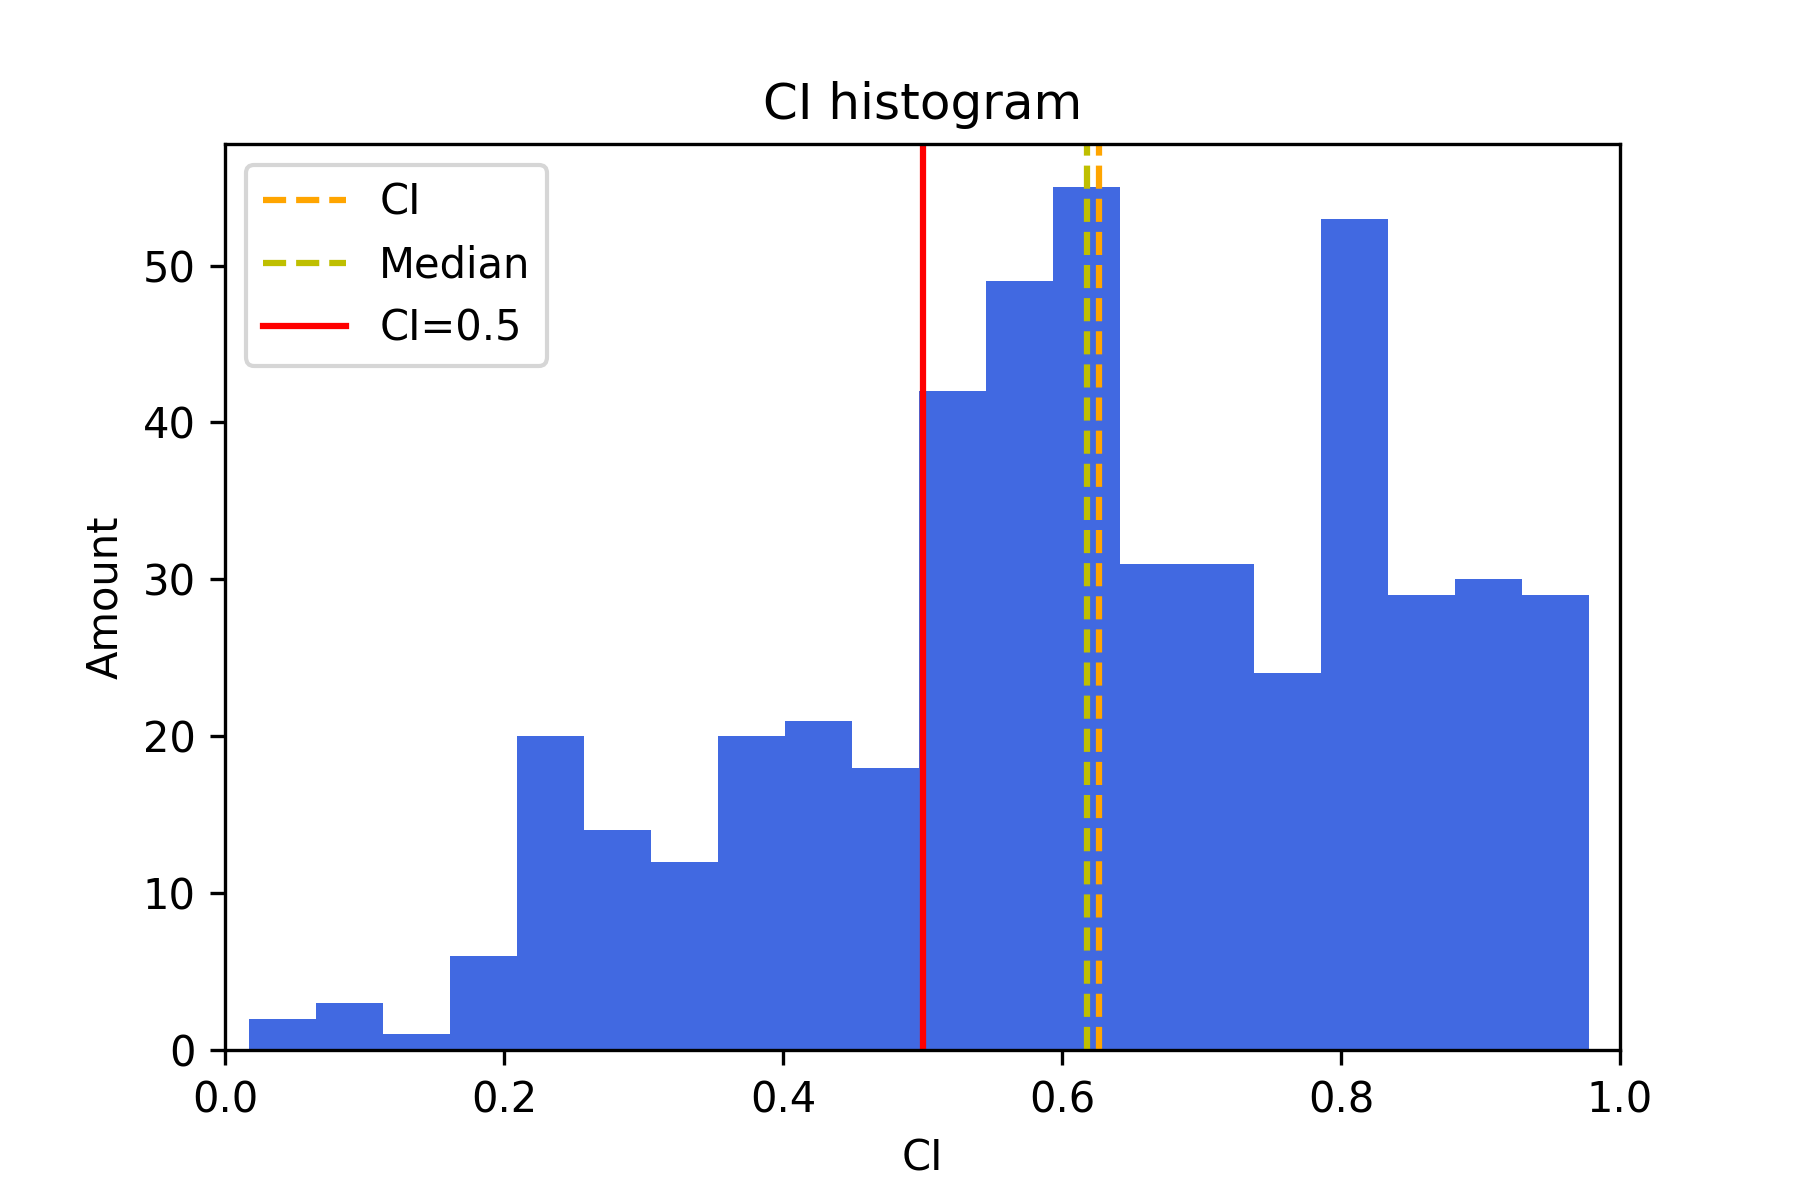
\includegraphics[width=.8\textwidth]{images/results/c-index_volume}
  \caption[LOOCV volume only model results]{
    Volume only model results using \acrshort{LOOCV} \label{fig:results-volume-LOOCV}
    
    Histogram showing the distribution of all the \acrshort{LOOCV} elements' \acrshort{CI}
    when using mixed pairs to obtain the \acrshort{CI}. Final \gls{CI} is 0,627, median
    \gls{CI} is 0,618.
  }
\end{figure}

\ssecc{Build shallow siamese network}
\label{sec:shallow-siamese}

The initial shallow siamese network design had a very simple design for the sister network. 
In fact, it was so simple that a proper \gls{CNN} could not be build, the original design 
can be found in \autoref{fig:shallow-sister}.

The main problem was that there were only two convolutional layers so that when trying to reduce
the image dimension the output image still was too big for a Fully Connected layer. With this
problem in mind a new design was made and it's shown in \autoref{fig:shallow-implement}.

This new design has more layers to reduce the dimensions of the image and is able to 
incorporate the scalar data. As it was previously said this design it's still part of the
siamese network model.

This task took two weeks to complete and no further development will be held with this task
since the next efforts are centered around a model using only the radiomic features.

\begin{figure}
  \centering
  
\begin{tikzpicture}[every node/.style={scale=.8}]

  \tikzstyle{module}=[rounded corners, draw, align=center]
  \tikzstyle{FC}=[module, fill=green!30]
  \tikzstyle{conv}=[module, fill=orange!30]
  \tikzstyle{io}=[module, fill=purple!30]
  
  
  \node [io] (image) {Image};
  \node [conv, below = of image] (CNN-1) at (0, 0) {
    Convolution 1 \\ 
    \( 30 @ 3 \times 3 \times 3 \) \\
    Stride = 2
  };
  \node [conv, below = of CNN-1] (CNN-2) {
    Convolution 2 \\
    \( 30 @ 3 \times 3 \times 3 \) \\
    Stride = 2
  };
  \node [conv, below = of CNN-2] (CNN-3) {
    Convolution 3 \\
    \( 40 @ 3 \times 3 \times 3 \)
  };
  \node [conv, below = of CNN-3] (CNN-4) {
    Convolution 4 \\
    \( 40 @ 3 \times 3 \times 3 \)
  };
  \node [conv, below = of CNN-4] (CNN-5) {
    Convolution 5 \\
    \( 50 @ 3 \times 3 \times 3 \)
  };

  \node [right = 5 of image] (aux) {};
  \node [io, right = of aux] (scalar) {Scalar};

  \node [FC, below = of aux] (con) {Concatenate + \\ flatten};
  \node [left = of con] (aux-2) {};
  \node [FC, below = of con] (FC-1) {FC \\ 8000 units};
  \node [FC, below = of FC-1] (FC-2) {FC \\ 1000 units};
  \node [FC, below = of FC-2] (FC-3) {FC \\ 10 units};

  \node [io, below = of FC-3] (out) {Sister out};
  
  \draw [-latex] (image) -- (CNN-1) node[midway, right] {\( 64 \times 64 \times 64 \times 1 \)};
  \draw [-latex] (CNN-1) -- (CNN-2) node[midway, right] {\( 31 \times 31 \times 31 \times 30 \)};
  \draw [-latex] (CNN-2) -- (CNN-3) node[midway, right] {\( 15 \times 15 \times 15 \times 40 \)};
  \draw [-latex] (CNN-3) -- (CNN-4) node[midway, right] {\( 13 \times 13 \times 13 \times 40 \)};
  \draw [-latex] (CNN-4) -- (CNN-5) node[midway, right] {\( 11 \times 11 \times 11 \times 40 \)};

  \draw (CNN-5) -| (aux-2.center)  node[pos=.3, below] {\( 9 \times 9 \times 9 \times 50 \)};
  \draw [-latex] (aux-2.center) |- (con);
  \draw [-latex] (scalar) |- (con) node[pos=.15, left] {\( 725 \)};
  
  \draw [-latex] (con) -- (FC-1) node[midway, right] {\( 37.175 \)};
  \draw [-latex] (FC-1) -- (FC-2) node[midway, right] {\( 8000 \)};
  \draw [-latex] (FC-2) -- (FC-3) node[midway, right] {\( 1000 \)};
  \draw [-latex] (FC-3) -- (out) node[midway, right] {\( 10 \)};
\end{tikzpicture}



  \caption{Shallow siamese sister's network illustration \label{fig:shallow-implement}}
\end{figure}

\sssecc{Results}

The results have been obtained using 4-\gls{CV}. The training parameters where:
\begin{itemize}
  \item Learning rate: 0,001
  \item Regularization factor: 0,01
  \item Number of epochs: 10
  \item Batch size: 40
\end{itemize}
A bigger batch size could not be used because
the model was using a lot of memory. By having a small batch size the number of train 
iterations was of 2.180. The 4-\gls{CV} results can be seen at \autoref{tab:results-shallow-4CV}.

It can be seen that the number of pairs is not the same as in \autoref{tab:results-volume-4CV} 
from the volume model. This is caused by data augmentation. Since
data augmentation is used, there are four images for each patient so the number of pairs
increases too.

The results show a really poor performance, even poorer than random. So, these results
do not improve the current state-of-the-art and are worse than the results that have 
been set to create a baseline. 

It's interesting to highlight that the network has not even learned what it had learned in the 
previous design even being the volume one of the radiomic features
that are passed as input.

\begin{table}
  \centering
  \begin{tabular}{|c||c|c|c||c|c|c|}
    \cline{2-7}
    \multicolumn{1}{c|}{} & \multicolumn{3}{|c||}{\textbf{Pairs}} & 
    \multicolumn{3}{c|}{\textbf{Concordance Index}} \\
    \hline
    \textbf{Fold} & \textbf{Mixed} & \textbf{Train} & \textbf{Test} & 
    \textbf{Mixed} & \textbf{Train} & \textbf{Test} \\
    \hhline{=======}
    0 & 65.436 & 187.216 & 21.320 & 0,43 & 0,42 & 0,419 \\
    1 & 65.436 & 187.828 & 21.112 & 0,444 & 0,431 & 0,459 \\
    2 & 65.392 & 190.308 & 20.336 & 0,472 & 0,474 & 0,426 \\
    3 & 65.392 & 189.096 & 20.704 & 0,514 & 0,512 & 0,514 \\
    \hhline{=======}
    \textbf{Total} & 261.656 & 754.448 & 83.472 & 0,465 & 0,459 & 0,455 \\
    \hline
  \end{tabular}

  \caption[Shallow 4-CV results]{
    Results for shallow model using 4-CV \label{tab:results-shallow-4CV}.
  }
\end{table}

\ssecc{Build scalar only siamese network}
\label{sec:scalar-only}

To speed up the testing process, a siamese network that only used scalar features 
was built. With this approach, the training time was reduced from around 5 hours 
to 1 minute to train a single model. 

To improve the network's performance Dropout \cite{neural:dropout} was used, by using 
dropout some of the model activations are zeroed and then scaled according to the 
dropout probability. This way, the networks' neurons do not have all the information and 
thus they must generalize. Dropout is used as a way of regularization. 

Moreover, since this model inherits from the basic model, defined in \autoref{sec:basic-siamese}, 
regularization is applied too by adding the l2 norm of the weights. The loss and
cost functions are the same too.

To complete this step it took one week but two more weeks were needed to validate the results 
and to fix some bugs.

\begin{figure}
  \centering
  
\begin{tikzpicture}[every node/.style={scale=.8}]

  \tikzstyle{module}=[rounded corners, draw, align=center]
  \tikzstyle{FC}=[module, fill=green!30]
  \tikzstyle{conv}=[module, fill=orange!30]
  \tikzstyle{io}=[module, fill=purple!30]

  \node [io] (scalar) {Scalar};

  \node [FC, right = of scalar] (FC-1) {FC \\ 500 units \\ tanh};
  \node [conv, right = of FC-1] (D-1) {Dropout \\ 20\%};
  \node [FC, right = of D-1] (FC-2) {FC \\ 200 units \\ tanh};
  \node [conv, right = of FC-2] (D-2) {Dropout \\ 20\%};

  \node [FC, below = of FC-1] (FC-3) {FC \\ 50 units \\ tanh};
  \node [conv, right = of FC-3] (D-3) {Dropout \\ 20\%};
  \node (aux) at ($(FC-3)!0.5!(FC-1)$) {};
  \node [FC, right = of D-3] (FC-4) {FC \\ 10 units \\ ReLu};


  \node [io, right = of FC-4] (out) {Sister out};
  \draw [-latex] (scalar) -- (FC-1) node[midway, below] {\( 725 \)};

  \draw [-latex] (FC-1) -- (D-1) node[midway, below] {\( 500 \)};
  \draw [-latex] (D-1) -- (FC-2) node[midway, below] {\( 500 \)};
  \draw [-latex] (FC-2) -- (D-2) node[midway, below] {\( 200 \)};
  
  \draw [-latex] (D-2) |- node[pos=.75, below]{\( 200 \)} (aux) -| (FC-3);
  \draw [-latex] (FC-3) -- (D-3) node[midway, below] {\( 50 \)};
  \draw [-latex] (D-3) -- (FC-4) node[midway, below] {\( 50 \)};
  \draw [-latex] (FC-4) -- (out) node[midway, below] {\( 10 \)};

  % \draw [-latex] (FC-3) -- (out) node[midway, below] {\( 10 \)};
\end{tikzpicture}



  \caption{Scalar siamese network illustration \label{fig:scalar-implement}}
\end{figure}

\sssecc{Results}

The results obtained with this model are both with 4-CV and \gls{LOOCV}. The training 
parameters have been the following ones:
\begin{itemize}
  \item Learning rate: 0,001
  \item Regularization factor: 0,01
  \item Dropout probability: 0,2/1
  \item Number of epochs: 1000
  \item Batch size: The whole dataset
\end{itemize}

A summary of the results using 4-CV can be seen at \autoref{tab:results-scalar-4CV}. It can be
observed that the number of pairs is not constant through all the folds. This is caused by
censoring, since not all members can form a pair with all the other ones some elements 
have more available pairs than others. 

From the 4-CV results it can be seen that the final test \gls{CI} is 0,635 and the final mixed 
\gls{CI} is 0,764. Even thought it seems that the test results are very similar to the
state-of-the art (0,628) when compared to the baseline the test results are similar but
the mixed pairs results have improved (0,764 vs 0,616).

The improvement with the baseline is relevant because the final objective of the project
is to create a model to predict a patient's survival time. The final method to predict
survival will be to compare a new patient against the whole training set and then, having
all the comparisons and the survival time of the train set's patients, a prediction of
the new patient's survival time can will be made. This means that the most relevant 
indicator is the mixed \gls{CI}.

The results using \gls{LOOCV} can be seen represented in \autoref{fig:results-scalar-LOOCV}. 
In this case, only the mixed pairs have been compared to create the histogram.

The final \gls{CI} with \gls{LOOCV} is 0,771 while the median \gls{CI} is 0,862. The final 
\gls{CI} using \gls{LOOCV} is very similar to the one obtained using 4-CV (0,771 vs 0,764).

\begin{table}
  \centering
  \begin{tabular}{|c||c|c|c||c|c|c|}
    \cline{2-7}
    \multicolumn{1}{c|}{} & \multicolumn{3}{|c||}{\textbf{Pairs}} & 
    \multicolumn{3}{c|}{\textbf{Concordance Index}} \\
    \hline
    \textbf{Fold} & \textbf{Mixed} & \textbf{Train} & \textbf{Test} & 
    \textbf{Mixed} & \textbf{Train} & \textbf{Test} \\
    \hhline{=======}
    0 & 16.359 & 46.804 & 5.330 & 0,728 & 0,915 & 0,543 \\
    1 & 16.359 & 46.957 & 5.278 & 0,809 & 0,927 & 0,64 \\
    2 & 16.348 & 47.577 & 5.084 & 0,751 & 0,91 & 0,675 \\
    3 & 16.348 & 47.274 & 5.176 & 0,766 & 0,919 & 0,624 \\
    \hhline{=======}
    \textbf{Total} & 65.414 & 188.612 & 20.868 & 0,764 & 0,918 & 0,62   \\
    \hline
  \end{tabular}

  \caption[Scalar Only 4-CV results]{
    Results for scalar only model using 4-CV \label{tab:results-scalar-4CV}
  }
\end{table}

\begin{figure}
  \centering
  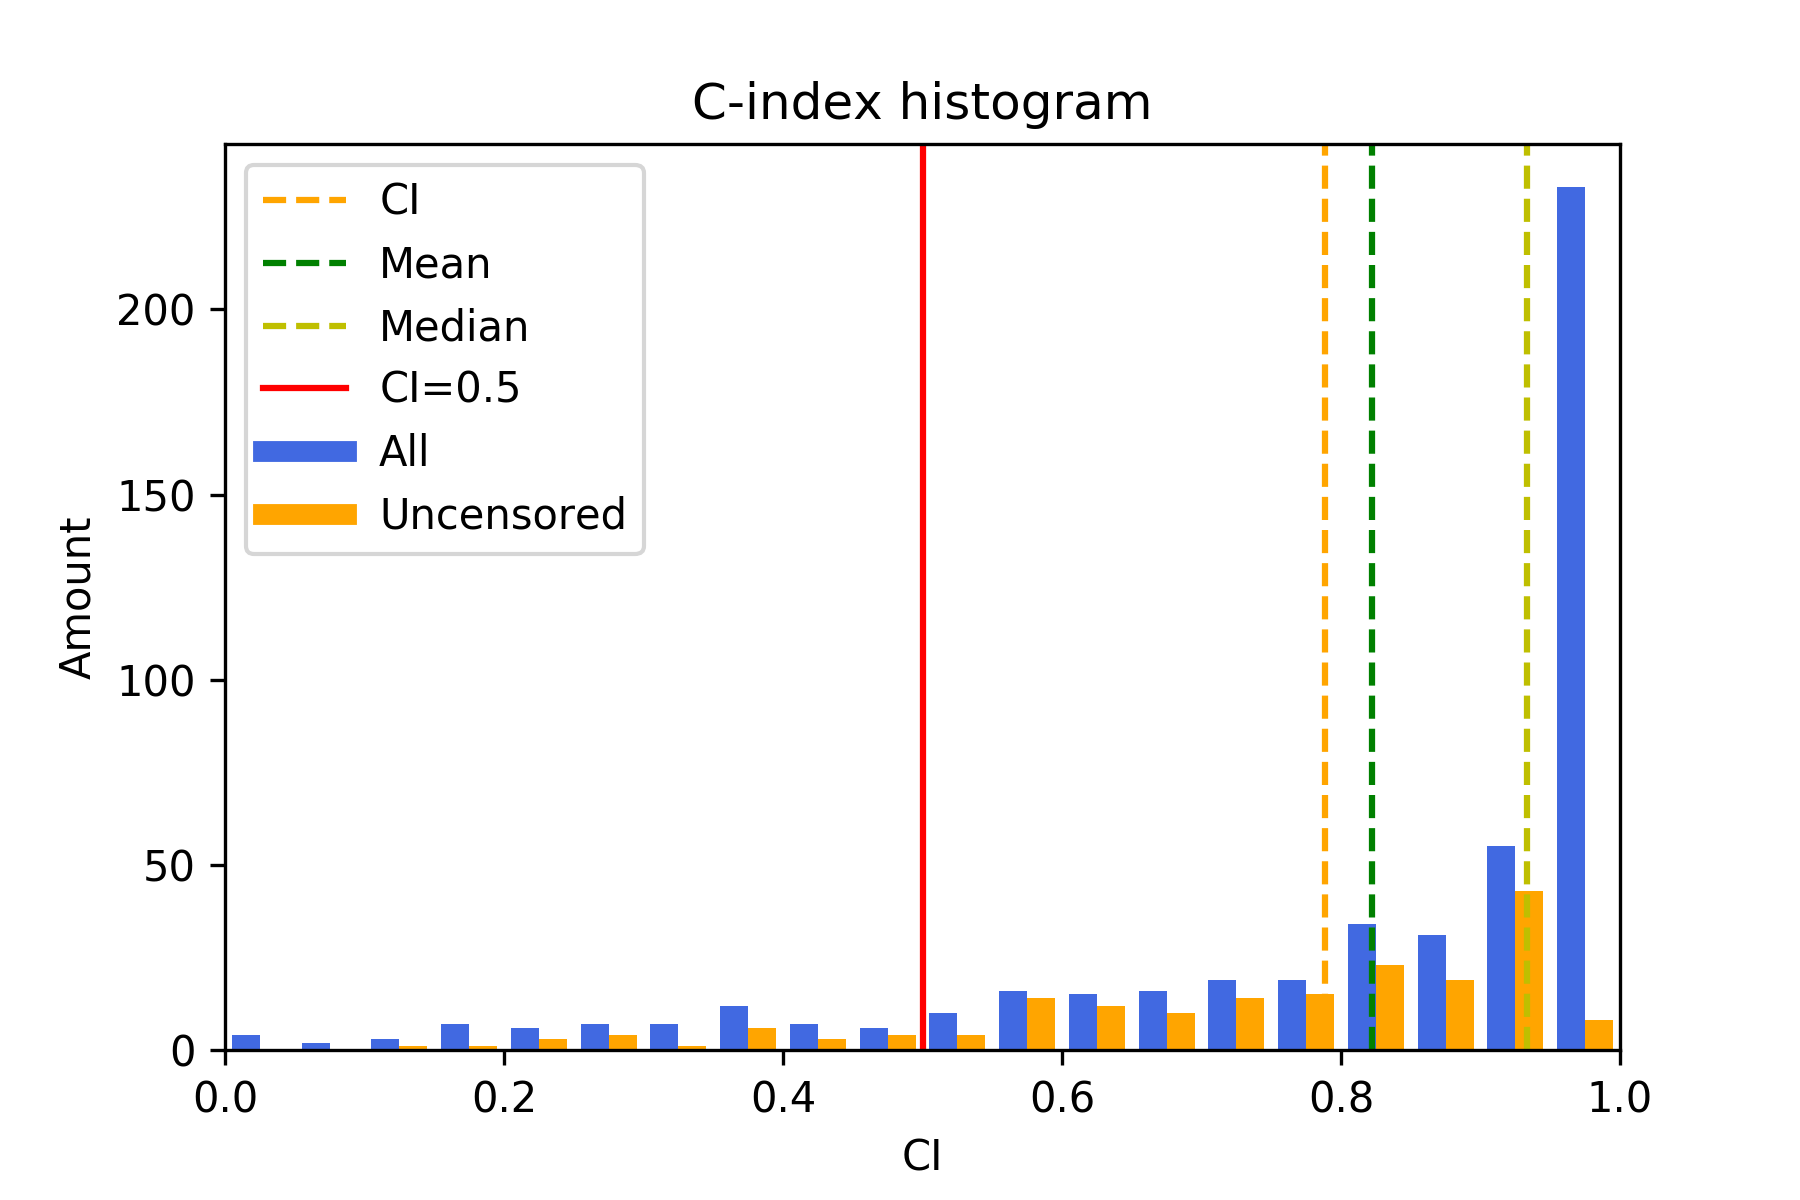
\includegraphics[width=.8\textwidth]{images/results/c-index_scalar}
  \caption[LOOCV scalar only model results]{
    Scalar only model results using \acrshort{LOOCV} \label{fig:results-scalar-LOOCV}
    
    Histogram showing the distribution of all the \acrshort{LOOCV} elements' \acrshort{CI}
    when using mixed pairs to obtain the \acrshort{CI}. Final \gls{CI} is 0,771, median 
    \gls{CI} is 0,862.
  }
\end{figure}

\ssecc{Build deep siamese network}

The deep siamese network design is derived by the Shallow Siamese design shown in 
\autoref{sec:shallow-siamese} although it has more convolutional layers and defines 
multiple types of blocks that are used through the network. As the previous design,
it uses both the radiomic scalar features and the images extracted from the \gls{CT} 
scans. 

Moreover, the design is also inspired in Inception-ResNet-v1 which in turn is 
inspired in Inception-v4 \cite{neural:inception-4}. The whole network's structure can be 
seen in \autoref{fig:residual-general}.

The network is composed by a total of seven convolutional blocks, a final
pooling layer and three more fully connected layers where the radiomic scalar features are
injected. Only the Stem (\autoref{fig:residual-block-stem}), 
Reduction A (\autoref{fig:residual-block-reduce-a}) and
Reduction B (\autoref{fig:residual-block-reduce-b}) blocks reduce the image dimensions,
while the A (\autoref{fig:residual-block-a}) and B (\autoref{fig:residual-block-b}) 
blocks are useful to learn deep features.

\begin{figure}
  \centering
  
\begin{tikzpicture}[every node/.style={scale=.8}]

  \tikzstyle{module}=[rounded corners, draw, align=center]
  \tikzstyle{FC}=[module, fill=green!30]
  \tikzstyle{conv}=[module, fill=orange!30]
  \tikzstyle{io}=[module, fill=purple!30]
  
  
  \node [io] (image) {Image};

  \node [conv, below = of image] (S) {Stem bloc};
  \node [conv, below = of S] (BA) {2 x Block A 1};
  \node [conv, below = of BA] (R-A) {Reduction A};
  \node [conv, below = of R-A] (BB) {2 x Block B};
  \node [conv, below = of BB] (R-B) {Reduction B};
  \node [conv, below = of R-B] (P) {
    Average pooling \\
    \( 350 @ 6 \times 6 \times 6 \)
  };

  \node [right = 5 of image] (aux) {};
  \node [io, right = of aux] (scalar) {Scalar};

  \node [FC, below = of aux] (con) {Concatenate + \\ flatten};
  \node [left = of con] (aux-2) {};
  \node [FC, below = of con] (FC-1) {FC \\ 800 units};
  \node [FC, below = of FC-1] (FC-2) {FC \\ 100 units};
  \node [FC, below = of FC-2] (FC-3) {FC \\ 10 units};

  \node [io, below = of FC-3] (out) {Sister out};

  \draw [-latex] (image) -- (S) node[midway, right] {\( 64 \times 64 \times 64 \times 1 \)};
  \draw [-latex] (S) -- (BA) node[midway, right] {\( 31 \times 31 \times 31 \times 50 \)};
  \draw [-latex] (BA) -- (R-A) node[midway, right] {\( 31 \times 31 \times 31 \times 50 \)};
  \draw [-latex] (R-A) -- (BB) node[midway, right] {\( 15 \times 15 \times 15 \times 130 \)};
  \draw [-latex] (BB) -- (R-B) node[midway, right] {\( 15 \times 15 \times 15 \times 130 \)};
  \draw [-latex] (R-B) -- (P) node[midway, right] {\( 7 \times 7 \times 7 \times 350 \)};

  \draw (P) -| (aux-2.center)  node[pos=.3, below] {\( 2 \times 2 \times 2 \times 350 \)};
  \draw [-latex] (aux-2.center) |- (con);
  \draw [-latex] (scalar) |- (con) node[pos=.15, left] {\( 725 \)};
  
  \draw [-latex] (con) -- (FC-1) node[midway, right] {\( 3.525 \)};
  \draw [-latex] (FC-1) -- (FC-2) node[midway, right] {\( 800 \)};
  \draw [-latex] (FC-2) -- (FC-3) node[midway, right] {\( 100 \)};
  \draw [-latex] (FC-3) -- (out) node[midway, right] {\( 10 \)};
\end{tikzpicture}



  \caption[Deep siamese network main structure]{
    Deep siamese network main structure \label{fig:residual-general}
    
    The drawing represents the design used for the sister network in the deep siamese
    network design.
  }
\end{figure}
\begin{figure}
  \centering
  \begin{subfigure}[b]{.4\textwidth}
    \centering
    \scalebox{.9}{
\begin{tikzpicture}[every node/.style={scale=.8}, node distance = 1.5 em]

  \tikzstyle{module}=[rounded corners, draw, align=center]
  \tikzstyle{FC}=[module, fill=green!30]
  \tikzstyle{conv}=[module, fill=orange!30]
  \tikzstyle{pool}=[module, fill=cyan!30]
  \tikzstyle{io}=[module, fill=purple!30]
  \tikzstyle{tensor}=[font=\scriptsize\selectfont]
  
  
  \node [io] (image) {Image};

  \node [conv, below left = 0.5 and 1 of image.south] (A) {
    Convolution \\
    \( 25 @ 3 \times 3 \times 3 \) \\
    Stride = 2
  };
  \node [pool, below right = 0.5 and 1 of image.south] (B-0) {
    Max  Pooling \\
    \( 1 @ 3 \times 3 \times 3 \) \\
    Stride = 2
  };
  \node [conv, below = of B-0] (B-1) {
    Convolution \\
    \( 25 @ 1 \times 1 \times 1 \) \\
    Same padding
  };

  \node [FC, below left = .5 and 1 of B-1.south] (con) {Concatenate};
  \node [io, below = of con] (out) {Stem out};

  \draw [-latex] (image) -| (A) node[tensor, midway, above] {\( 64 \times 64 \times 64 \times 1 \)};
  \draw [-latex] (image) -| (B-0) node[tensor, midway, above] {\( 64 \times 64 \times 64 \times 1 \)};
  \draw [-latex] (B-0) -- (B-1) node[tensor, midway, left] {\( 31 \times 31 \times 31 \times 1 \)};
  \draw [-latex] (B-1) |- (con) node[tensor, near start, left] {\( 31 \times 31 \times 31 \times 25 \)};
  \draw [-latex] (A) |- (con) node[tensor, near start, right] {\( 31 \times 31 \times 31 \times 25 \)};
  \draw [-latex] (con) -- (out) node[tensor, midway, left] {\( 31 \times 31 \times 31 \times 50 \)};

\end{tikzpicture}


}
    \caption{Residual network Stem Block \label{fig:residual-block-stem}}
  \end{subfigure}
  \hfill
  \begin{subfigure}[b]{.59\textwidth}
    \centering
    \scalebox{.9}{
\begin{tikzpicture}[every node/.style={scale=.8}]

  \tikzstyle{module}=[rounded corners, draw, align=center]
  \tikzstyle{FC}=[module, fill=green!30]
  \tikzstyle{conv}=[module, fill=orange!30]
  \tikzstyle{io}=[module, fill=purple!30]
  
  
  \node [io] (image) {Input};

  \node [conv, below = of image] (B-C-0) {
    Convolution \\
    \( 32 @ 1 \times 1 \times 1 \) \\
    Same padding
  };
  \node [conv, below = of B-C-0] (B-C-1) {
    Convolution \\
    \( 1 @ 3 \times 3 \times 3 \) \\
    Same padding
  };

  \node [conv, left = of B-C-0] (A-C) {
    Convolution \\
    \( 32 @ 1 \times 1 \times 1 \) \\
    Same padding
  };
  \node [conv, right = of B-C-0] (C-C-0) {
    Convolution \\
    \( 32 @ 1 \times 1 \times 1 \) \\
    Same padding
  };
  \foreach \x [remember=\x as \lastx (initially 0)] in {1,2} {
    \node [conv, below = of C-C-\lastx] (C-C-\x) {
      Convolution \\
      \( 32 @ 3 \times 3 \times 3 \) \\
      Same padding
    };
  }

  \node [FC, below = 3 of B-C-1] (con) {Concatenate};
  
  \node [conv, below = of con] (F-C) {
    Convolution \\
    \( 50 @ 1 \times 1 \times 1 \) \\
    Same padding
    };
  \node [circle, FC, below = of F-C] (sum) {\LARGE +};
  \node [io, below = of sum] (out) {Block A out};

  \node [right = of C-C-0] (aux) {};

  \draw [-latex] (image) -| (A-C) node[midway, above] {\( 31 \times 31 \times 31 \times 50 \)};
  \draw [-latex] (image) -- (B-C-0) node[midway, left] {\( 31 \times 31 \times 31 \times 50 \)};
  \draw [-latex] (image) -| (C-C-0) node[midway, above] {\( 31 \times 31 \times 31 \times 50 \)};

  \draw [-latex] (B-C-0) -- (B-C-1) node[midway, left] {\( 31 \times 31 \times 31 \times 32 \)};
  \draw [-latex] (C-C-0) -- (C-C-1) node[midway, left] {\( 31 \times 31 \times 31 \times 32 \)};
  \draw [-latex] (C-C-1) -- (C-C-2) node[midway, left] {\( 31 \times 31 \times 31 \times 32 \)};

  \draw [-latex] (A-C) |- (con) node[near start, right] {\( 31 \times 31 \times 31 \times 32 \)};
  \draw [-latex] (B-C-1) -- (con) node[midway, left] {\( 31 \times 31 \times 31 \times 32 \)};
  \draw [-latex] (C-C-2) |- (con) node[near start, left] {\( 31 \times 31 \times 31 \times 32 \)};

  \draw [-latex] (con) -- (F-C) node[midway, left] {\( 31 \times 31 \times 31 \times 96 \)};
  \draw [-latex] (F-C) -- (sum) node[midway, left] {\( 31 \times 31 \times 31 \times 50 \)};
  \draw (image) -| (aux.center);
  \draw [-latex] (aux.center) |- (sum) node[near end, above] {\( 31 \times 31 \times 31 \times 50 \)};
  \draw [-latex] (sum) -- (out) node[midway, left] {\( 31 \times 31 \times 31 \times 50 \)};

\end{tikzpicture}


}
    \caption{Residual network convolutional Block A \label{fig:residual-block-a}}
  \end{subfigure}
  \caption{Residual Network blocks}
\end{figure}

\begin{figure}\ContinuedFloat
  \begin{subfigure}[b]{.55\textwidth}
    \centering
    \scalebox{.85}{
\begin{tikzpicture}[every node/.style={scale=.8}, node distance = 0.7]

  \tikzstyle{module}=[rounded corners, draw, align=center]
  \tikzstyle{FC}=[module, fill=green!30]
  \tikzstyle{conv}=[module, fill=orange!30]
  \tikzstyle{pool}=[module, fill=cyan!30]
  \tikzstyle{io}=[module, fill=purple!30]
  \tikzstyle{tensor}=[font=\scriptsize\selectfont]
  
  
  \node [io] (image) {Input};

  \node [conv, below = 0.5 and 1 of image] (B-0) {
    Convolution \\
    \( 50 @ 3  \times 3 \times 3 \) \\
    Same padding
  };

  \node [pool, left = of B-0] (A) {
    Max Pooling \\
    \( 32 @ 3 \times 3 \times 3 \) \\
    Stride = 2
  };
  \node [conv, right = of B-0] (C-0) {
    Convolution \\
    \( 30 @ 1 \times 1 \times 1 \) \\
    Same padding
  };
  \node [conv, below = of C-0] (C-1) {
    Convolution \\
    \( 30 @ 3 \times 3 \times 3 \) \\
    Same padding
  };
  \node [conv, below = of C-1] (C-2) {
    Convolution \\
    \( 30 @ 3 \times 3 \times 3 \) \\
    Stride = 2
  };

  \node (aux-1) at ($(C-2 -| B-0) + (0, -.5)$) {};

  \node [FC, below = of aux-1] (con) {Concatenate};
  \node [io, below = of con] (out) {Reduction A out};

  \draw [-latex] (image) -| (A) node[tensor, near start, above] {\( 31 \times 31 \times 31 \times 50 \)};
  \draw [-latex] (image) -- (B-0) node[tensor, midway, left] {\( 31 \times 31 \times 31 \times 50 \)};
  \draw [-latex] (image) -| (C-0) node[tensor, near start, above] {\( 31 \times 31 \times 31 \times 50 \)};

  \draw [-latex] (C-0) -- (C-1) node[tensor, midway, left] {\( 31 \times 31 \times 31 \times 30 \)};
  \draw [-latex] (C-1) -- (C-2) node[tensor, midway, left] {\( 31 \times 31 \times 31 \times 30 \)};

  \draw [-latex] (A) |- (con) node[tensor, near start, right] {\( 15 \times 15 \times 15 \times 50 \)};
  \draw [-latex] (B-0) -- (con) node[tensor, near start, left] {\( 15 \times 15 \times 15 \times 50 \)};
  \draw [-latex] (C-2) |- (con) node[tensor, near start, left] {\( 15 \times 15 \times 15 \times 30 \)};

  \draw [-latex] (con) -- (out) node[tensor, midway, left] {\( 15 \times 15 \times 15 \times 130 \)};

\end{tikzpicture}


}
    \caption{Residual network Reduction A \label{fig:residual-block-reduce-a}}
  \end{subfigure}
  \begin{subfigure}[b]{.44\textwidth}
    \centering
    \scalebox{.85}{
\begin{tikzpicture}[every node/.style={scale=.8}, node distance = 0.7]

  \tikzstyle{module}=[rounded corners, draw, align=center]
  \tikzstyle{FC}=[module, fill=green!30]
  \tikzstyle{conv}=[module, fill=orange!30]
  \tikzstyle{pool}=[module, fill=cyan!30]
  \tikzstyle{io}=[module, fill=purple!30]
  \tikzstyle{tensor}=[font=\scriptsize\selectfont]
  
  
  \node [io] (image) {Input};

  \node [conv, below = 0.5 of image] (B-C-0) {
    Convolution \\
    \( 50 @ 1 \times 1 \times 1 \) \\
    Same padding
  };
  \node [conv, below = of B-C-0] (B-C-1) {
    Convolution \\
    \( 50 @ 1  \times 1 \times 7 \) \\
    Same padding
  };
  \node [conv, below = of B-C-1] (B-C-2) {
    Convolution \\
    \( 50 @ 1  \times 7 \times 1 \) \\
    Same padding
  };
  \node [conv, below = of B-C-2] (B-C-3) {
    Convolution \\
    \( 50 @ 7  \times 1 \times 1 \) \\
    Same padding
  };

  \node [conv, left = of B-C-0] (A-C) {
    Convolution \\
    \( 50 @ 1 \times 1 \times 1 \) \\
    Same padding
  };

  \node [right = of B-C-0] (aux-1) {};

  \node [FC, below = of B-C-3] (con) {Concatenate};

  \node [conv, below = of con] (F-C) {
    Convolution \\
    \( 130 @ 1 \times 1 \times 1 \) \\
    Same padding
    };
  \node [circle, FC, below = of F-C] (sum) {\LARGE +};

  \node [io, below = of sum] (out) {Reduction A out};

  \draw [-latex] (image) -| (A-C) node[tensor, midway, above] {\( 15 \times 15 \times 15 \times 130 \)};
  \draw [-latex] (image) -- (B-C-0) node[tensor, midway, left] {\( 15 \times 15 \times 15 \times 130 \)};
  
  \draw [-latex] (A-C) |- (con) node[tensor, midway, below] {\( 15 \times 15 \times 15 \times 50 \)};
  \draw [-latex] (B-C-0) -- (B-C-1) node[tensor, midway, left] {\( 15 \times 15 \times 15 \times 50 \)};
  \draw [-latex] (B-C-1) -- (B-C-2) node[tensor, midway, left] {\( 15 \times 15 \times 15 \times 50 \)};
  \draw [-latex] (B-C-2) -- (B-C-3) node[tensor, midway, left] {\( 15 \times 15 \times 15 \times 50 \)};
  \draw [-latex] (B-C-3) -- (con) node[tensor, midway, left] {\( 15 \times 15 \times 15 \times 50 \)};
  
  \draw (image) -| (aux-1.center);
  \draw [-latex] (aux-1.center) |- (sum) node[tensor, midway, below] {\( 15 \times 15 \times 15 \times 130 \)};
  
  \draw [-latex] (F-C) -- (sum) node[tensor, midway, left] {\( 15 \times 15 \times 15 \times 130 \)};
  \draw [-latex] (con) -- (F-C) node[tensor, midway, left] {\( 15 \times 15 \times 15 \times 100 \)};
  \draw [-latex] (sum) -- (out) node[tensor, midway, left] {\( 15 \times 15 \times 15 \times 130 \)};

\end{tikzpicture}


}
    \caption{Residual network Block B \label{fig:residual-block-b}}
  \end{subfigure}

  \begin{subfigure}[b]{\textwidth}
    \centering
    \scalebox{.9}{
\begin{tikzpicture}[every node/.style={scale=.8}, node distance = 0.7, x=2.5em, y=2.5em]

  \tikzstyle{module}=[rounded corners, draw, align=center,]
  \tikzstyle{FC}=[module, fill=green!30]
  \tikzstyle{conv}=[module, fill=orange!30]
  \tikzstyle{pool}=[module, fill=cyan!30]
  \tikzstyle{io}=[module, fill=purple!30]
  \tikzstyle{tensor}=[font=\scriptsize\selectfont]
  
  
  \node [io] (image) {Input};

  \node [conv, below left = .5 and .5 of image.center] (B-0) {
    Convolution \\
    \( 100 @ 1 \times 1 \times 1 \) \\
    Same padding
  };
  \node [conv, below = of B-0] (B-1) {
    Convolution \\
    \( 100 @ 3 \times 3 \times 3 \) \\
    Stride = 2
  };

  \node [conv, left = of B-0] (A) {
    Convolution \\
    \( 100 @ 3 \times 3 \times 3 \) \\
    Stride = 2
  };

  \node [conv, below right = .5 and .5 of image.center] (C-0) {
    Convolution \\
    \( 100 @ 1 \times 1 \times 1 \) \\
    Same padding
  };

  \node [conv, below = of C-0] (C-1) {
    Convolution \\
    \( 100 @ 3 \times 3 \times 3 \) \\
    Stride = 2
  };

  \node [conv, right = of C-0] (D-0) {
    Convolution \\
    \( 50 @ 1 \times 1 \times 1 \) \\
    Same padding
  };

  \node [conv, below = of D-0] (D-1) {
    Convolution \\
    \( 50 @ 3 \times 3 \times 3 \) \\
    Same padding
  };

  \node [conv, below = of D-1] (D-2) {
    Convolution \\
    \( 50 @ 3 \times 3 \times 3 \) \\
    Stride = 2
  };

  \node (aux-1) at ($(D-2 -| C-1) + (0, -.5)$) {};

  \node [FC, below left = .5 and .5 of aux-1.south] (con) {Concatenate};
  \node [io, below = of con] (out) {Block B out};

  \draw [-latex] (image) -| (A);
  \draw [-latex] (image) -| (B-0) node[tensor, midway, above] {\( 15 \times 15 \times 15 \times 130 \)};
  \draw [-latex] (image) -| (C-0) node[tensor, midway, above] {\( 15 \times 15 \times 15 \times 130 \)};
  \draw [-latex] (image) -| (D-0);
  
  \draw [-latex] (A) |- (con) node[tensor, midway, below] {\( 7 \times 7 \times 7 \times 100 \)};

  \draw [-latex] (B-0) -- (B-1) node[tensor, midway, left] {\( 15 \times 15 \times 15 \times 100 \)};
  \draw [-latex] (B-1) |- (con) node[tensor, near start, left] {\( 7 \times 7 \times 7 \times 100 \)};
  
  \draw [-latex] (C-0) -- (C-1) node[tensor, midway, left] {\( 15 \times 15 \times 15 \times 100 \)};
  \draw [-latex] (C-1) |- (con) node[tensor, near start, left] {\( 7 \times 7 \times 7 \times 100 \)};
  
  \draw [-latex] (D-0) -- (D-1) node[tensor, midway, left] {\( 15 \times 15 \times 15 \times 50 \)};
  \draw [-latex] (D-1) -- (D-2) node[tensor, midway, left] {\( 15 \times 15 \times 15 \times 50 \)};
  \draw [-latex] (D-2) |- (con) node[tensor, midway, below] {\( 7 \times 7 \times 7 \times 50 \)};

  \draw [-latex] (con) -- (out) node[tensor, midway, left] {\( 7 \times 7 \times 7 \times 350 \)};

\end{tikzpicture}


}
    \caption{Residual network Block B \label{fig:residual-block-reduce-b}}
  \end{subfigure}
  \caption{Residual Network blocks (continuation)}
\end{figure}

\sssecc{Results}

To get the results for the deep siamese network 4-\gls{CV} has been used. The training
parameters are the following ones:
\begin{itemize}
  \item Learning rate: 0,001
  \item Regularization factor: 0,01
  \item Dropout probability: 0,2/1
  \item Number of epochs: 15
  \item Batch size: 20
\end{itemize}

The results with this training can be seen in \autoref{tab:results-residual-4CV}, the final
mixed \gls{CI} is 0,601 while the final train \gls{CI} is 0,603.
As it can be seen in \autoref{fig:results-residual-CI} only two of the four folds have 
properly converged to a solution when training the residual model, while the other two folds
have stayed in a random \gls{CI}. The two folds that have properly converged have been able
to obtain an average mixed \gls{CI} of 0,793 which is similar to the results using only
the scalar radiomic features (0,793 vs 0,771).

Future work on this task will be to find the proper hyper-parameters to make sure that all
the folds can finally converge and then train the model using \gls{LOOCV} to make sure
that not only certain distributions are able to show this behavior.

\begin{table}
  \centering
  \begin{tabular}{|c||c|c|c||c|c|c|}
    \cline{2-7}
    \multicolumn{1}{c|}{} & \multicolumn{3}{|c||}{\textbf{Pairs}} & 
    \multicolumn{3}{c|}{\textbf{Concordance Index}} \\
    \hline
    \textbf{Fold} & \textbf{Mixed} & \textbf{Train} & \textbf{Test} & 
    \textbf{Mixed} & \textbf{Train} & \textbf{Test} \\
    \hhline{=======}
    0 & 65.436 & 187.216 & 21.320 & 0,765 & 0,812 & 0,814 \\
    1 & 65.436 & 187.828 & 21.112 & 0,821 & 0,813 & 0,813 \\
    2 & 65.392 & 190.308 & 20.336 & 0,427 & 0,431 & 0,387 \\
    3 & 65.392 & 189.096 & 20.704 & 0,389 & 0,359 & 0,428 \\
    \hhline{=======}
    \textbf{Total} & 261.656 & 754.448 & 83.472 & 0,601 & 0,603 & 0,614 \\
    \hline
  \end{tabular}

  \caption[Residual 4-CV results]{
    Results for residual model using 4-CV \label{tab:results-residual-4CV}
  }
\end{table}

\begin{figure}
  \centering
  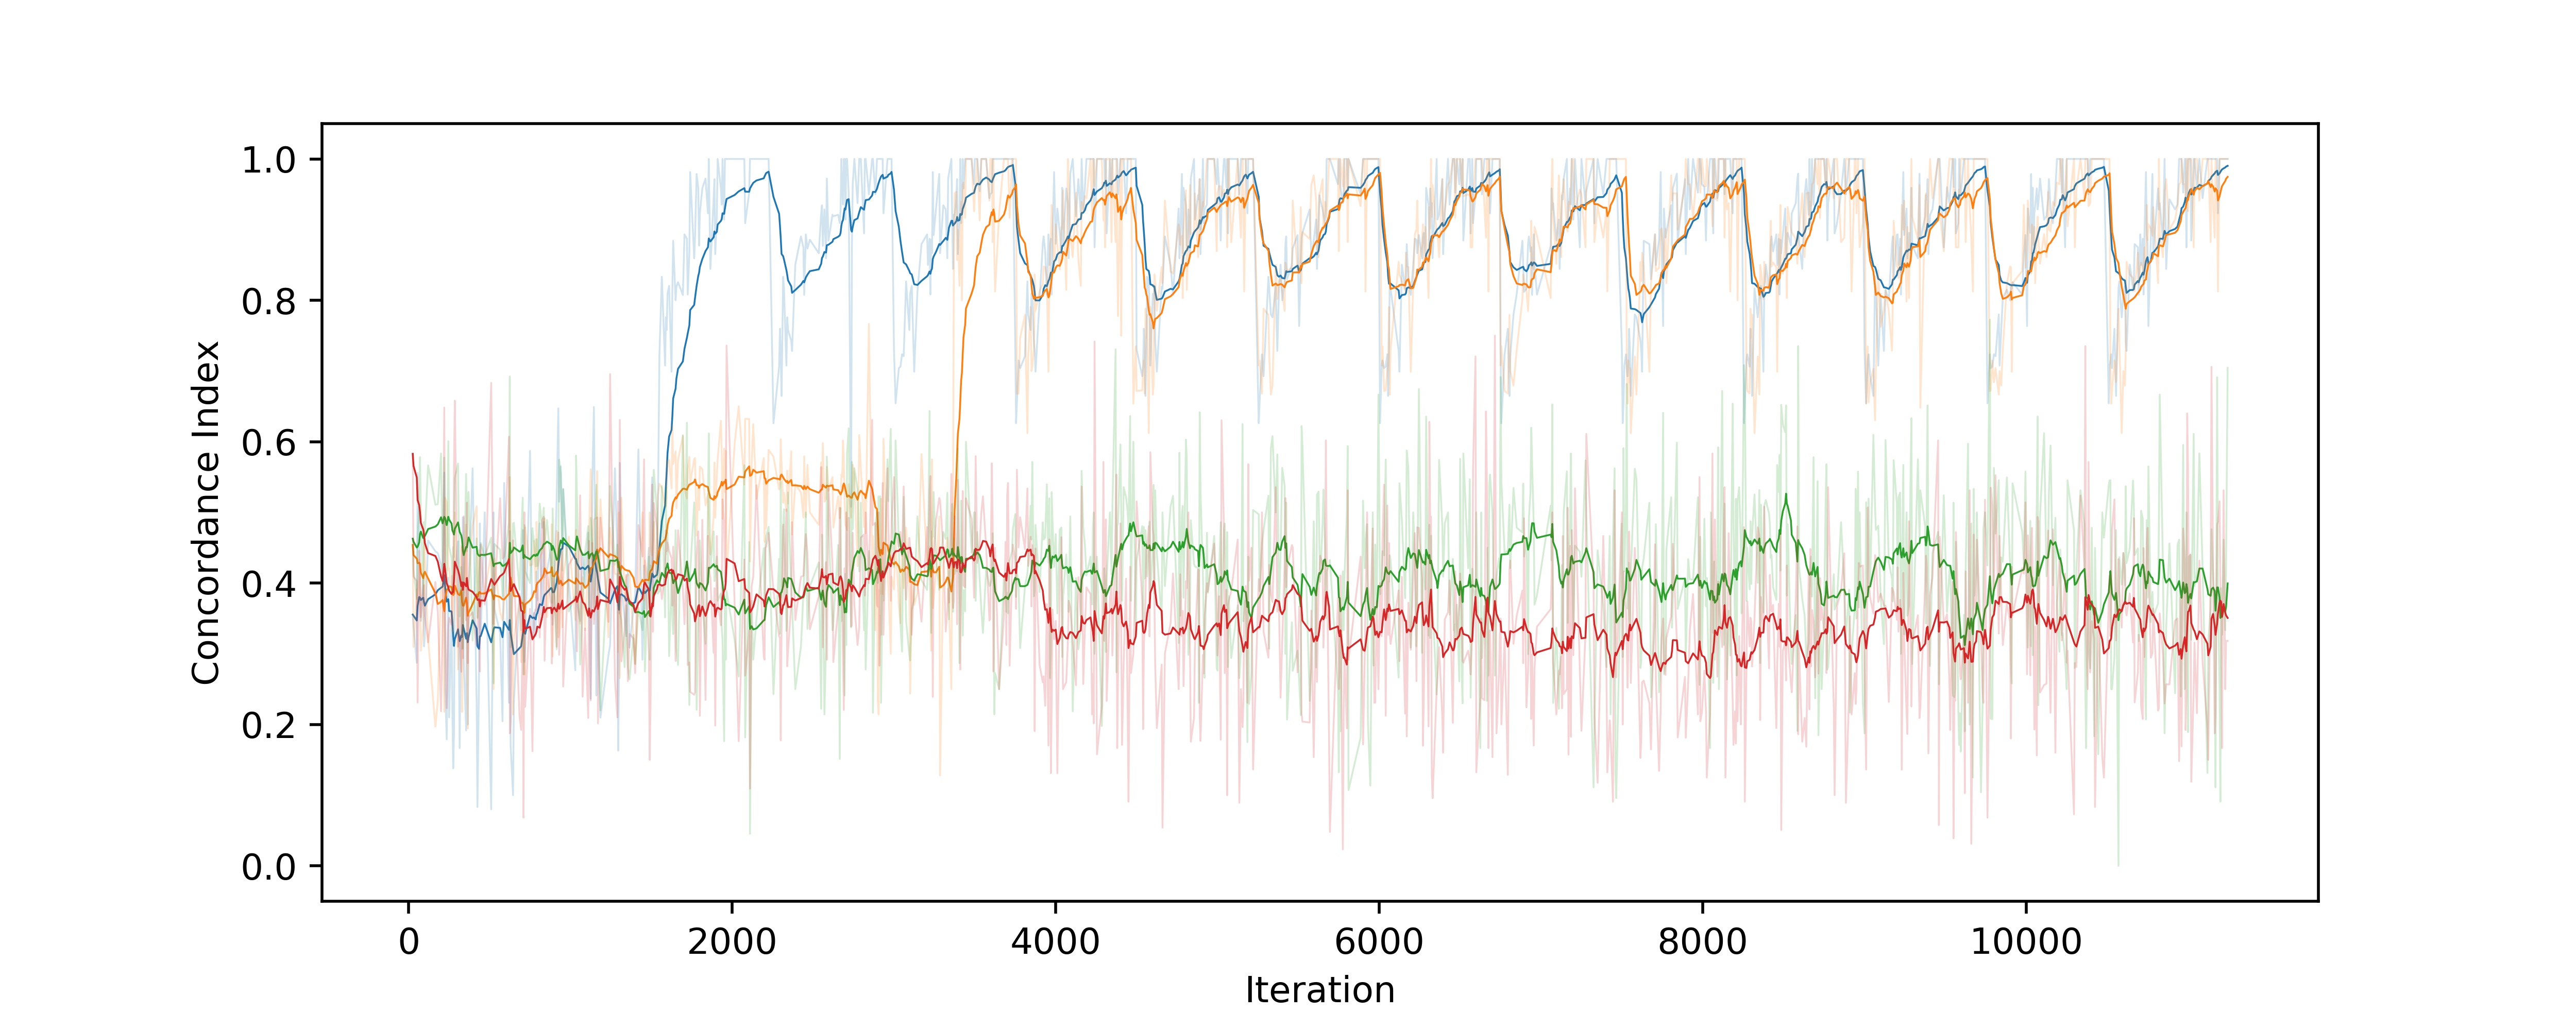
\includegraphics[width=\textwidth]{images/results/residual_train}

  \caption[Training iterations \gls{CI}]{
    \gls{CI} during training iterations of the deep residual model for each one of the 
    4-\gls{CV} folds. Each color represents a different fold. The real data is shown 
    in a lighter color, as some smoothing has been applied to show the tendency.

    \label{fig:results-residual-CI}
  }
\end{figure}

\ssecc{Predict patients survival}

Once one of the siamese models is working the next step is to predict a patient's survival
time. A basic approach would be to predict if they will be a long or short survival time 
patient. Multiple ideas have been brainstormed although not all of them have been tested.

The difficulty of the problem resides in sorting a test element at its proper position 
by using the comparison function \( T_A < T_B \) that the siamese network provides. 
The handicap is that, as it has been previously shown, this function gives the correct 
result 76,4\% of the time but fails the other 23,6\%, based on \autoref{sec:scalar-only} 
results. This means that a classical sorting algorithm, like merge sort, cannot be 
used since these type of algorithms are based in a comparison function with 100\% of accuracy.

A first approach was to divide the training set by setting a threshold at 2 years
and divide the set in long survivors and short survivors. Then compare each patient from the
test set against the long survivors and the short survivors. If the patient survives less
than the long survivors 70\% of the time then they will be classified as a short survivor and
as a long survivor if otherwise. Results using this method can be seen at 
\autoref{fig:survival-confusion}, final accuracy is 60\% while random accuracy is 50\%.

\begin{figure}
  \centering
  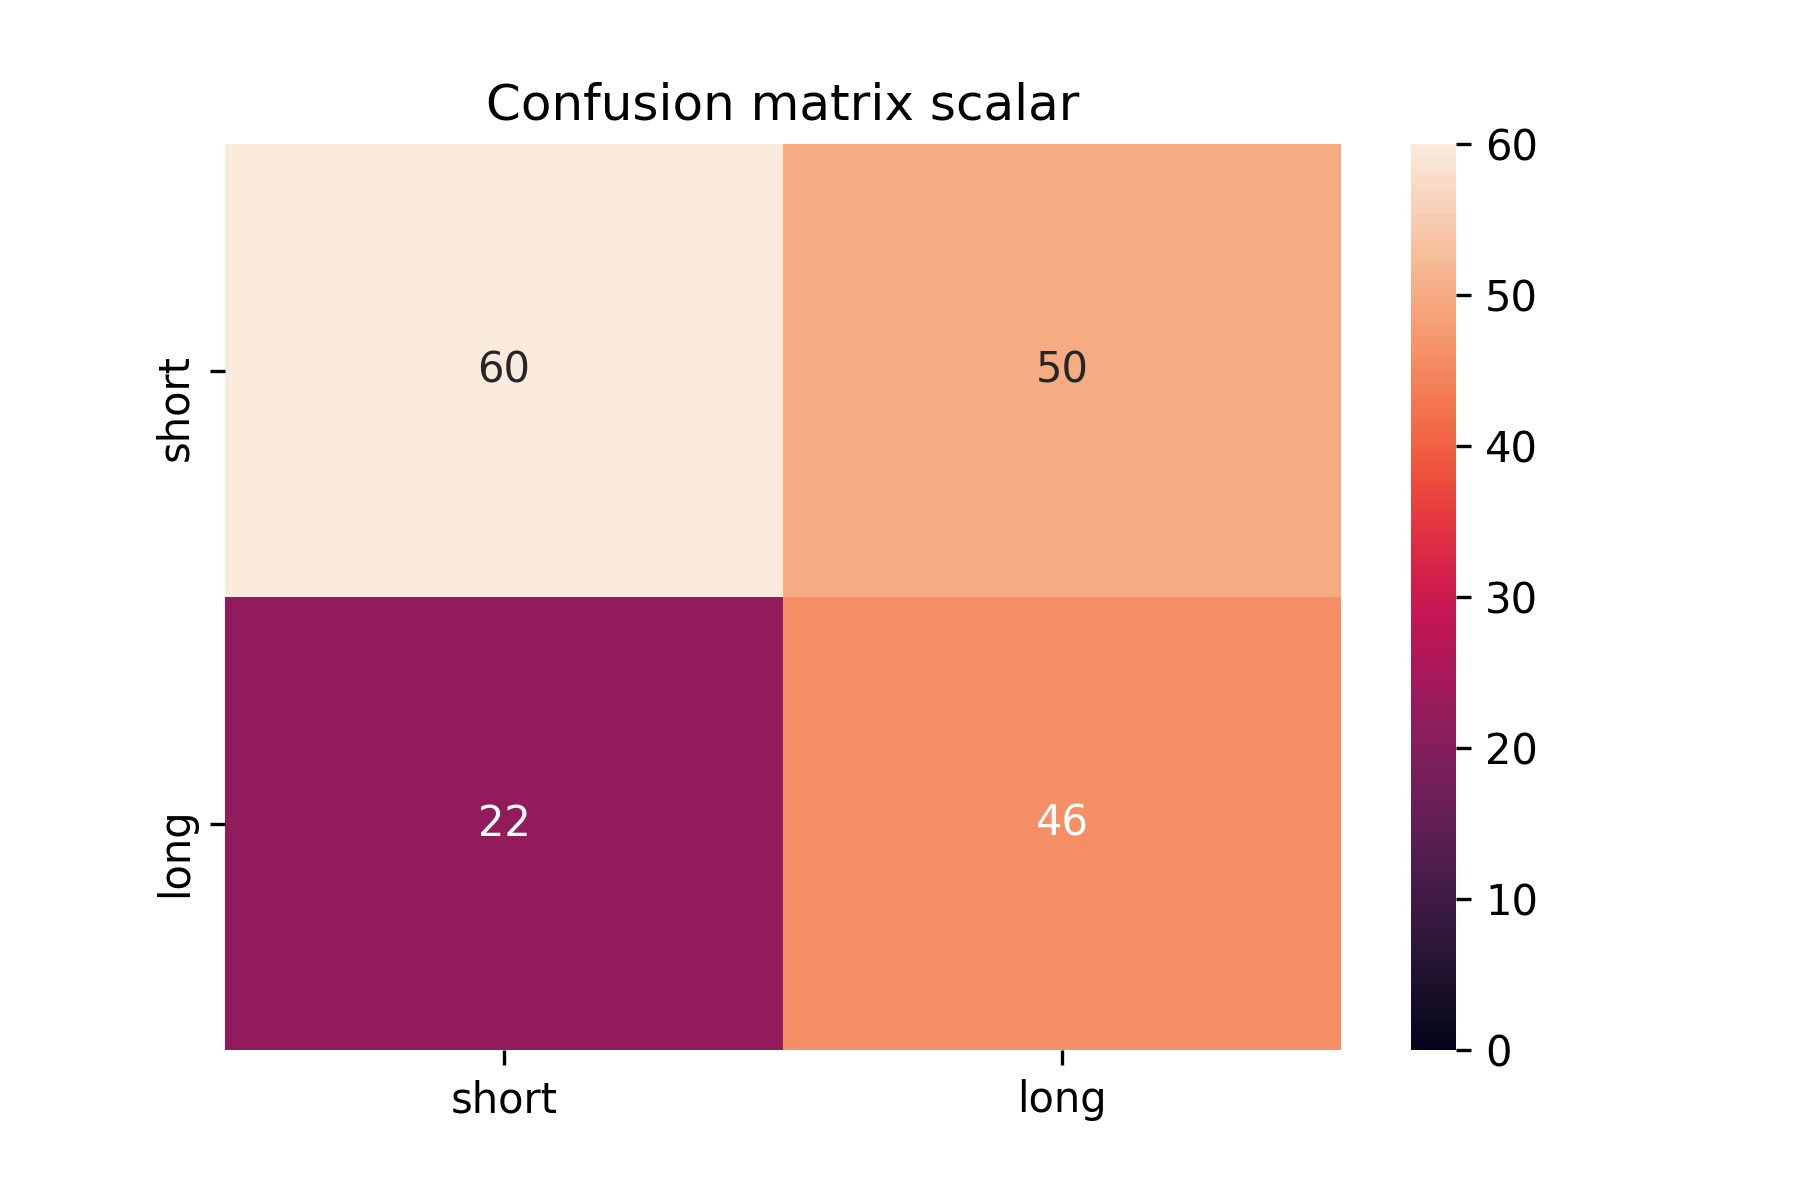
\includegraphics[width=.5\textwidth]{images/results/survival_scalar}

  \caption[Confusion matrix for survival classification]{
    Confusion matrix for survival classification between long survivors and short 
    survivors when using the results from \autoref{sec:scalar-only} that only uses
    radiomic scalar features. Final accuracy is 60\% (106 / 178).
    \label{fig:survival-confusion}
  }
\end{figure}

Since these results are not quite satisfying, future work will be to improve this step.
To do so, the next idea is to use the extracted features from the sister network output,
instead of the siamese network output, and then train a \gls{CPH} model using these features.

This way the siamese network is used to convert the regression problem into a classification 
problem and train a model with it. Then by extracting the hidden features the model can be
converted again into a regression model, already trained.

\ssecc{Write documentation}

Since this project creates a software, some documentation for the software must be written.
Moreover documenting the code is important to allow more people to work on the project.
The project's documentation can be found at \url{https://jmigual.github.io/CNNSurv/}.

This task has taken one week to complete, although some work has already been done while 
writing the code to make the task easier.

